\section{Paths Paranoia (More Recursion?)}{\label{sec:paths}}
\begin{topics}
\verb!recurrence relations! and previous sections.
\end{topics}	
\subsection{Staircase Walk}{\label{pp:staircasewalk}}
Consider a grid with $m$ horizontal lines and $n$ vertical lines. A Staircase Walk is defined as the path from bottom-left corner of the grid to the top right corner by walking along the lines; so, the person is constrained to move only in positive $x$ or positive $y$ direction.
\begin{figure}[H]
	\centering
	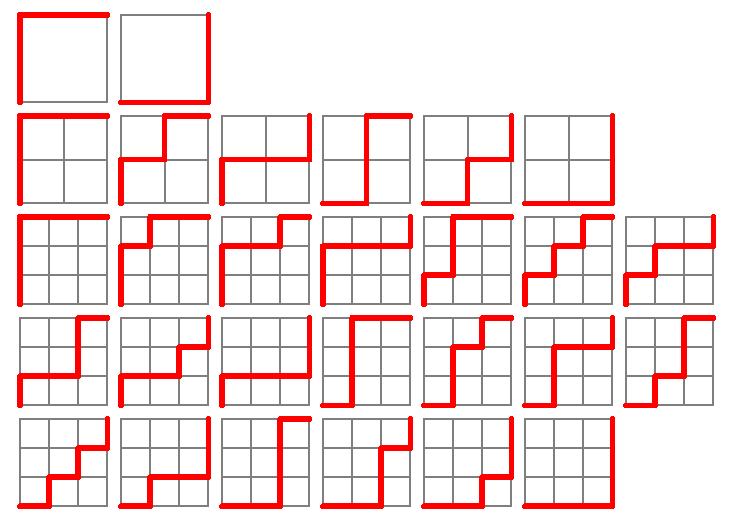
\includegraphics[width = 0.4\linewidth]{Staircase Walk.pdf}
	\caption{Example walks for case $m=n=1\ (\#2),\ m=n=2\ (\#6),\ m=n=3\ (\#20)$ (\href{https://mathworld.wolfram.com/StaircaseWalk.html}{Image Source})}
	\label{fig:staircasewalk}
\end{figure}
\vspace{-1em}
\textbf{Problem Statement:}\\
Find the number of possible \emph{Staircase Walks} for a given $m,n$ (for all test cases).
\begin{testcasesFunction}
	{$t$ \hfill(number of test cases, an integer)\\
	$m_1\ n_1\ \quad m_2\ n_2\ \quad \ldots\quad m_t\ n_t$ \hfill($t$ space seperated integer pairs for each testcase)}
	{Number of Staircase Walks for $m_i, n_i$  \hfill(each test case on a newline)}
	{$1 \leq m_i, n_i \leq 15$}
	{\texttt{int staircase\_walks(int m, int n)} -- returns the number of staircase walks for $m,n$.}
	{6\\1 1\quad 2 5\quad 6 3\quad 7 10\quad 13 8\quad15 15}
	% {11\\1 1\quad 2 2\quad 3 3\quad 5 5\quad 10 10\quad 15 15\quad 2 5\quad 3 3\quad 6 3\quad 7 10\quad 17 8\quad}
	{1\\5\\21\\5005\\50388\\40116600}
	{https://github.com/paramrathour/CS-101/tree/main/Starter Codes/Staircase Walk.cpp}
\end{testcasesFunction}
\begin{funvideo}
\href{https://youtu.be/dQXVn7pFsVI}{The Devil's Staircase -- PBS Infinite Series}\\
\href{https://youtu.be/LWPOlZBXtD8}{5 = 3 + 4? The Staircase Paradox. Spot The Mistake "Disproving" The Pythagorean Theorem -- Mind Your Decisions}
\end{funvideo}
\subsection{Dyck Path}{\label{pp:dyckpath}}
A Dyck Path is \hyperref[pp:staircasewalk]{Staircase Walk} ($m=n$) when the path always stays \emph{on or below the diagonal}.
\begin{figure}[H]
	\centering
	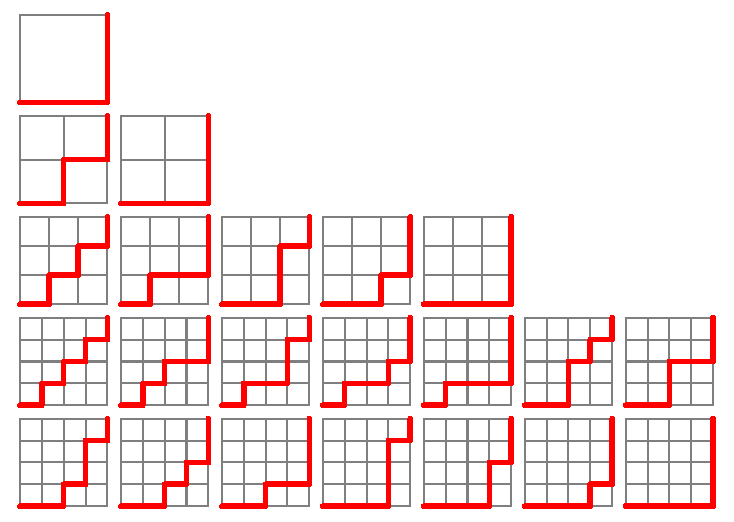
\includegraphics[width = 0.4\linewidth]{Dyck Path.pdf}
	\caption{Example walks for case $n=1\ (\#1),\ n=2\ (\#2),\ n=3\ (\#5), \ n=4\ (\#14)$ (\href{https://mathworld.wolfram.com/DyckPath.html}{Image Source})}
	\label{fig:dyckpath}
\end{figure}
\vspace{-1em}
\textbf{Problem Statement:}\\
Find the number of possible \emph{Dyck Path} for a given $n$ (for all test cases).
\begin{testcasesFunction}
	{$t$ \hfill(number of test cases, an integer)\\
	$n_1\ n_2\ \ldots n_t$ \hfill($t$ space seperated integers for each testcase)}
	{Number of Dyck Paths for $n_i$  \hfill(each test case on a newline)}
	{$1 \leq n_i \leq 15$}
	{\texttt{int dyck\_paths(int n)} -- returns the number of possible staircase walks for $n$.}
	{15\\1 2 3 4 5 6 7 8 9 10 11 12 13 14 15}
	{1\\2\\5\\14\\42\\132\\429\\1430\\4862\\16796\\58786\\208012\\742900\\2674440\\9694845}
	{https://github.com/paramrathour/CS-101/tree/main/Starter Codes/Dyck Path.cpp}
\end{testcasesFunction}
\subsection{Delannoy Number}{\label{pp:delannoynumber}}
Consider a grid with $m$ horizontal lines and $n$ vertical lines. A Delannoy Number is defined as the path from bottom-left corner of the grid to the top right corner by walking along the lines \emph{or diagonally upwards}; so, the person is constrained to move only in positive $x$ or positive $y$ or positive $x-y$ (i.e. along $y=x$) direction.
\begin{figure}[H]
	\centering
	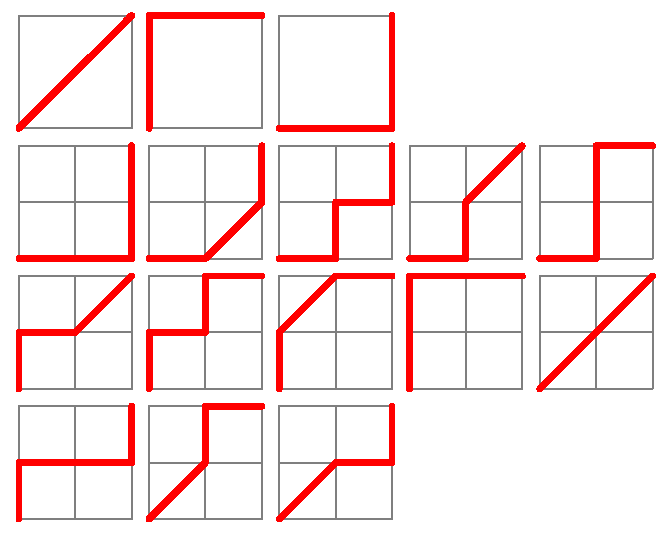
\includegraphics[width = 0.3\linewidth]{Delannoy Number.pdf}
	\caption{Example walks for case $m=n=1\ (\#2),\ m=n=2\ (\#6),\ m=n=3\ (\#20)$ (\href{https://mathworld.wolfram.com/DelannoyNumber.html}{Image Source})}
	\label{fig:delannoynumber}
\end{figure}
\vspace{-1em}
\textbf{Problem Statement:}\\
Find the number of possible \emph{Delannoy Numbers} for a given $m,n$ (for all test cases).
\begin{testcasesFunction}
	{$t$ \hfill(number of test cases, an integer)\\
	$m_1\ n_1\ \quad m_2\ n_2\ \quad \ldots\quad m_t\ n_t$ \hfill($t$ space seperated integer pairs for each testcase)}
	{Number of Delannoy Numbers for $m_i, n_i$  \hfill(each test case on a newline)}
	{$1 \leq m_i, n_i \leq 13$}
	{\texttt{int delannoy\_number(int m, int n)} -- returns the number of Delannoy Numbers for $m,n$.}
	% {6\\1 1\quad 2 5\quad 6 3\quad 7 10\quad 13 8\quad15 15}
	{11\\1 1\quad 2 2\quad 3 3\quad 5 5\quad 10 10\quad 13 13\quad 2 5\quad 3 3\quad 6 3\quad 7 10\quad 13 8}
	{3\\13\\63\\1683\\8097453\\1409933619\\61\\63\\377\\433905\\8405905}
	{https://github.com/paramrathour/CS-101/tree/main/Starter Codes/Delannoy Number.cpp}
\end{testcasesFunction}
\subsection{Schr\"oder Number}{\label{pp:schrodernumber}}
A Schroder Number is count of \hyperref[pp:delannoynumber]{Delannoy Walks} ($m=n$) when the path always stays \emph{on or below the diagonal}.
\begin{figure}[H]
	\centering
	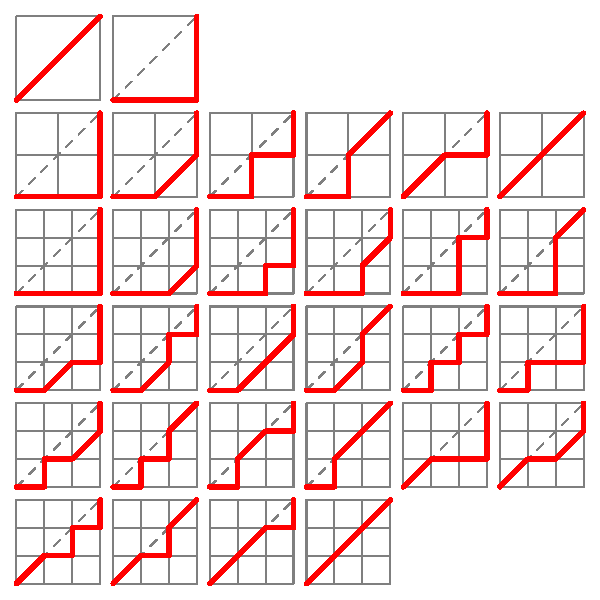
\includegraphics[width = 0.32\linewidth]{Schroder Number.pdf}
	\caption{Example walks for case $n=1\ (\#2),\ n=2\ (\#6),\ n=3\ (\#22)$ (\href{https://mathworld.wolfram.com/SchroederNumber.html}{Image Source})}
	\label{fig:schrodernumber}
\end{figure}
\vspace{-1.5em}
\textbf{Problem Statement:}\\
Find the \emph{Schroder Number} for a given $n$ (for all test cases).
\begin{testcasesFunction}
	{$t$ \hfill(number of test cases, an integer)\\
	$n_1\ n_2\ \ldots n_t$ \hfill($t$ space seperated integers for each testcase)}
	{Number of Schroder Numbers for $n_i$  \hfill(each test case on a newline)}
	{$1 \leq n_i \leq 14$}
	{\texttt{int schroder\_number(int n)} -- returns the number of possible delannoy walks for $n$.}
	{14\\1 2 3 4 5 6 7 8 9 10 11 12 13 14}
	{2\\6\\22\\90\\394\\1806\\8558\\41586\\206098\\1037718\\5293446\\27297738\\142078746\\745387038}
	{https://github.com/paramrathour/CS-101/tree/main/Starter Codes/Schroder Number.cpp}
\end{testcasesFunction}
\subsection{Motzkin Number}{\label{pp:motzkinnumber}}
Consider a grid with $n$ horizontal lines and $n$ vertical lines. A Motzkin Number is defined as the number of paths from bottom-left corner of the grid to the bottom-right corner which always stays on or above $x-$axis by walking horizontally fowards \emph{or diagonally upwards or diagonally downwards}; so, the person is constrained to move only in positive $x$ and along $y=x$ or $y=-x$ ($y$ direction can be negative).
\begin{figure}[H]
	\centering
	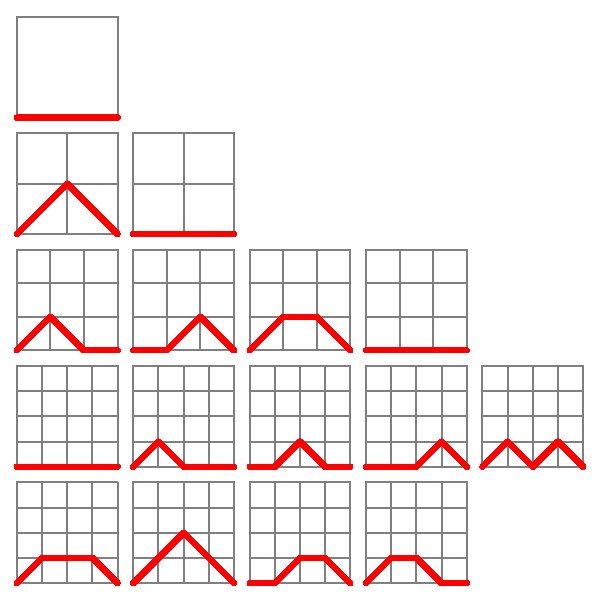
\includegraphics[width = 0.32\linewidth]{Motzkin Number.pdf}
	\caption{Example walks for case $n=1\ (\#1),\ n=2\ (\#2),\ n=3\ (\#4),\ n=4\ (\#9)$ (\href{https://mathworld.wolfram.com/MotzkinNumber.html}{Image Source})}
	\label{fig:motzkinnumber}
\end{figure}
\vspace{-1em}
\textbf{Problem Statement:}\\
Find the \emph{Motzkin Number} for a given $n$ (for all test cases).
\begin{testcasesFunction}
	{$t$ \hfill(number of test cases, an integer)\\
	$n_1\ n_2\ \ldots n_t$ \hfill($t$ space seperated integers for each testcase)}
	{Number of Motzkin Numbers for $n_i$  \hfill(each test case on a newline)}
	{$1 \leq n_i \leq 20$}
	{\texttt{int motzkin\_number(int n)} -- returns the number of possible walks for $n$.}
	{10\\1 2 3 4 5 8 11 14 17 20}
	{1\\2\\4\\9\\21\\323\\5798\\113634\\2356779\\50852019}
	{https://github.com/paramrathour/CS-101/tree/main/Starter Codes/Motzkin Number.cpp}
\end{testcasesFunction}
\subsection{Hilbert Curve}{\label{pp:hilbertcurve}}
\begin{figure}[H]
	\centering
	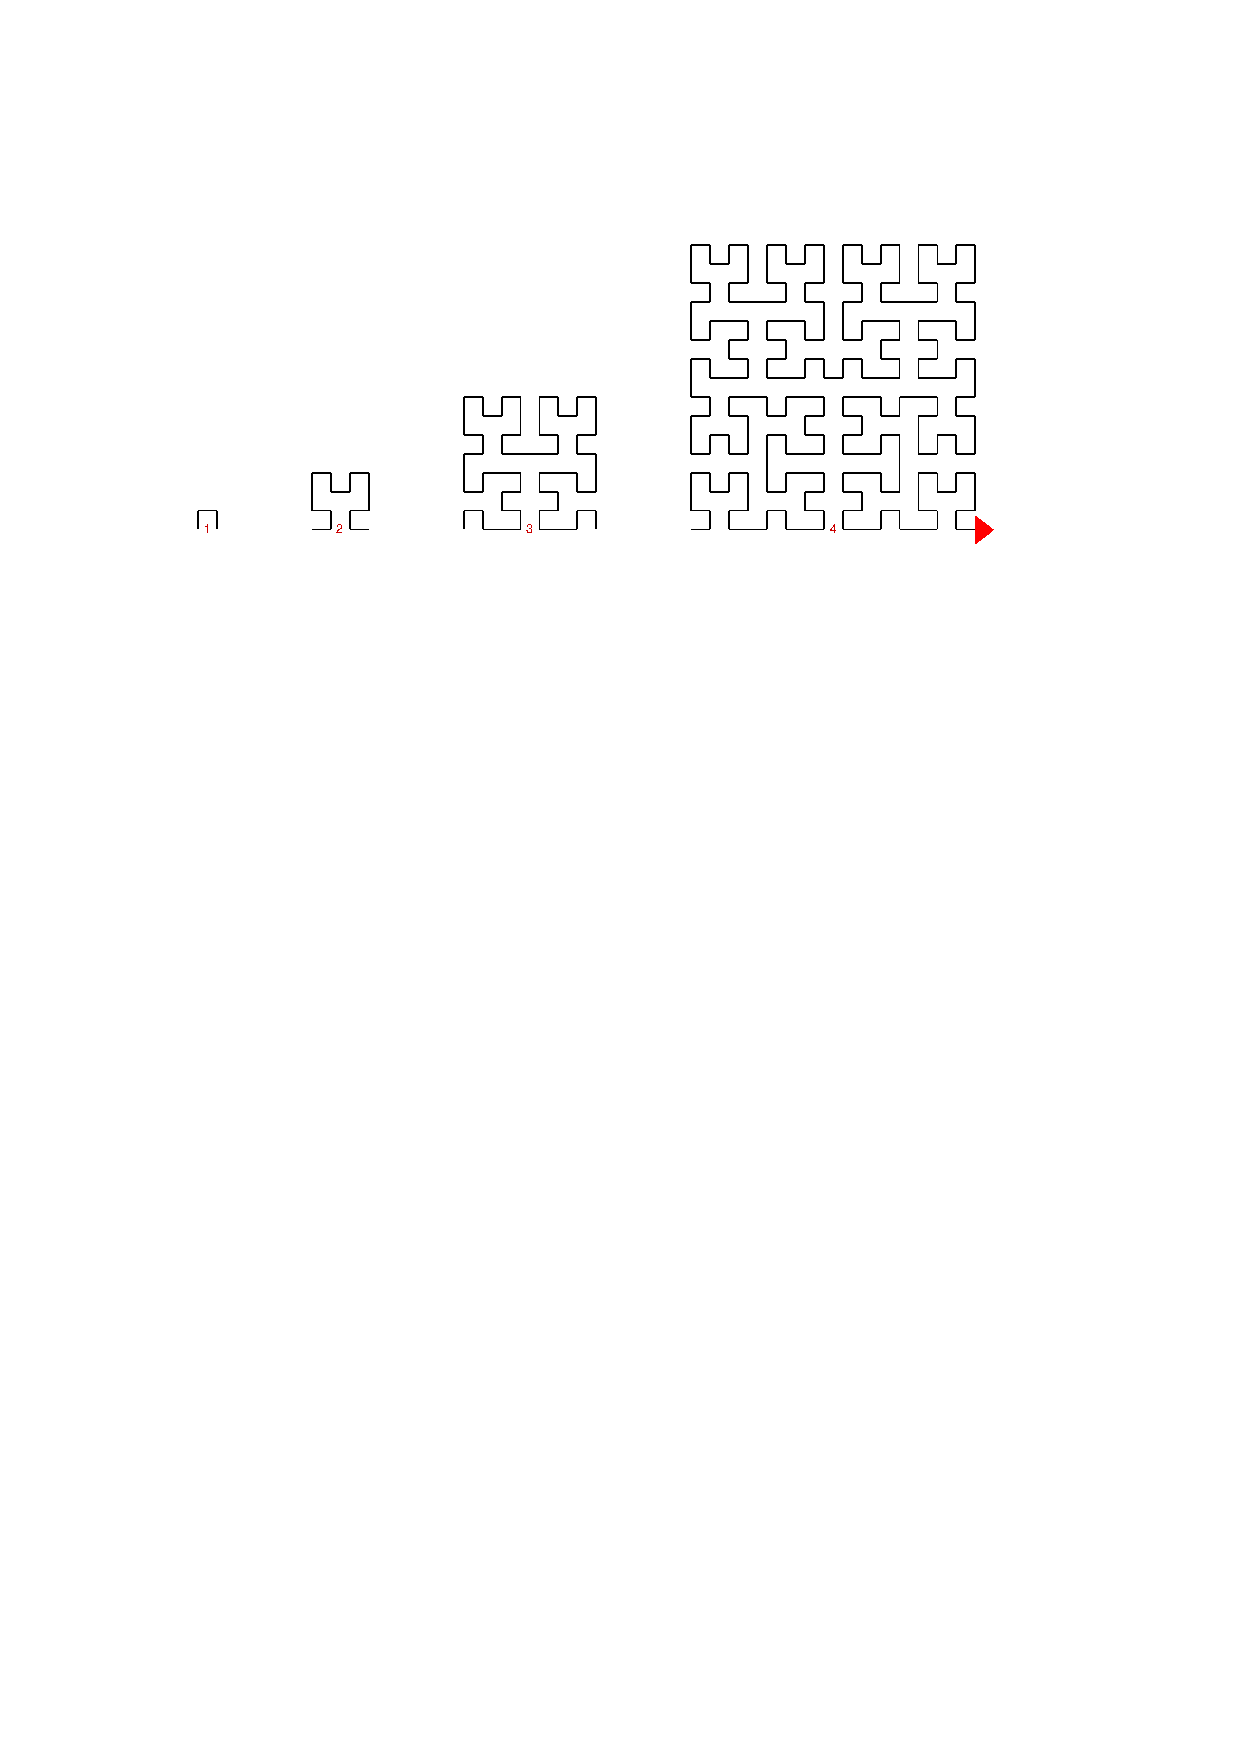
\includegraphics[width=\linewidth]{Hilbert Curve.pdf}
	\caption{Hilbert Curve (\href{https://www.cse.iitb.ac.in/~ranade/book.html}{Image Source})}
	\label{fig:hilbertcurve}
\end{figure}
\textbf{Problem Statement:}\\
Take an integer as input and draw the corresponding iteration of this fractal using \verb!turtleSim!\\
You may think along these lines
\begin{description}
	\item[Step 1]Find a simple pattern in these iterations.
	\item[Step 2]Think how can you implement this pattern in an efficient way (here think in the number of lines of code you have to write. \textbf{Word of caution}: this is just one of the possible definitions of efficient code).
	% \item[Step 3]Do you think that you need something that will implement/shorten your code?\\ How will it look like? (it’s a feature)
	\item[Step 3]Write the code!
\end{description}
In case you are stuck, here's the starter code!
\begin{tcolorbox}[breakable, enhanced, sharpish corners]%, colback = white]
	\href{https://github.com/paramrathour/CS-101/tree/main/Starter Codes/Hilbert Curve.cpp}{\textbf{Starter Code}}
\end{tcolorbox}
Feel free to discuss your thoughts.
\begin{funvideo}
\href{https://youtu.be/3s7h2MHQtxc}{Hilbert's Curve: Is infinite math useful? -- 3Blue1Brown}\\
\href{https://youtu.be/b-Fa6HtvGtQ}{Recursive PowerPoint Presentations [Gone Fractal!] -- Stand-up Maths}	
\end{funvideo}
For more interesting recursive and fractal problems, check out \hyperref[pp:lsystems]{L-Systems}.